\chapter{Photon Detector}
\label{ch:photon}
\section{Introduction}

Liquid argon is an excellent scintillating medium. With an average
energy needed to produce a photon of 19.5 eV (at zero field) a typical
1 MeV particle will generate 40,000 photons with 128 nm wavelength. At
higher fields this will be reduced but at 500 V/cm the yield is still
about $\sim$20,000 photons per MeV. Roughly 1/3 of the photons are
promptly emitted at around 6 ns and while the rest are are emitted
with a delay of 1100-1600 ns. LAr is highly transparent to the 128 VUV
photons with a Rayleigh scattering length and absorption length of 95
cm and >200 cm respectively. The relatively large light yield makes
the scintillation process an excellent candidate for determination of
$t_{0}$ for non-beam related events. Detection of the scintillation
light may also be helpful in background rejection.

\section{Requirements and Goals}

\subsection{Beam-based physics}

There are no requirements for the beam-based physics program, as the
machine clock will provide a $t_{0}$ with roughly 10 $\mu$s
resolution. Given that the electron drift is 1.6 mm/$\mu$s the
uncertainty to the electron lifetime correction is small is the beam
timing is used. The photon system can be useful in determining the
$t_{0}$ of cosmic ray events and events from radiological decays. The
impact of this on the detector performance needs to be determined, but
it is not expected that the reduction in backgrounds for the
oscillation program will introduce additional requirements to the
photon system design.

\subsection{Proton decay and atmospheric physics}

The photon detector system must provide the t0 for non-beam related
physics channels if a correction for electron recombination during
drift is to be applied. The requirements for electronics and hadronic
energy resolution for the proton decay and the atmospheric neutrino
program are $1\% / \sqrt{E(GeV)} \bigoplus 1\%$ and $30\% /
\sqrt{E(GeV)}$ respectively. With these resolutions the collected
charge must be accurately corrected for recombination. Therefore the
photon system must provide a $t_{0}$ for particles with >100 MeV with
>95\% efficiency in the fiducial volume of the detector.

\subsection{Low-energy physics}

Supernova events will produce neutrinos down to about $\sim$5
MeV. Studies have estimated the momentum resolution for 5 MeV
electrons to be 20\% using only TPC information and assuming a highly
efficient trigger and an electron lifetime of 5 ms. The impact of
various detector resolutions on the physics potential of LBNE has not
been studied in detail. At present there is no strong requirement that
the energy resolution must be better than 20\% so no requirement on
the photon system trigger efficiency is set at this time. However it
is clear that if a detector design can be found the energy resolution
would greatly improve. A goal of the photon detection R\&D is to
develop a system with the lowest possible threshold for a reasonable
cost. At time of the start of final design a final decision as to the
configuration will need to be made based on cost and added physics
capability.

\subsection{General Considerations}
In the event that larger photon collection efficiencies can be
achieved then it is possible to improve the energy resolution of the
detector by adding the photon yield to the electron yield information.
However this requires several orders of improvement in light
collection efficiency so it is beyond the scope of present designed.

\section{Photon Detector Prototype Designs}

All design considered for the photon detector have been based on the
use of wavelength-shifting coating, or bulk doping, of plastic
materials coupled to silicon photomultipliers (SiPMs). The reference
design~\ref{sec_bars} utilizes a coated acrylic waveguide coupled to
SiPMs. Alternatate designs, desribed in the following section, have
been developed to optimize coverage, cost, and attenuation length. 


\subsection{Cast or Bulk doped acrylic bars}
\label{sec_bars}

The reference design for the photon detection system is based on light
guides that are coated with wavelength shifter. The 128 nm
scintillation photons from liquid argon interact with the wavelength
shifter on the light guide surface and 430 nm light is re-emitted in
the bar.  The light guide channels the light to photodectors at its
end.

A schematic drawing of a light guide with its photosensors is shown in
Fig.~\ref{fig:WaveguideSketch}. The prototype light guides are bars
with a footprint 2.54 cm $\times$ 0.6 cm.  The concept is described in
Ref.~\cite{bib:MITbars}.
\begin{figure}[ht]
  \begin{center}
    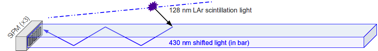
\includegraphics[width=.85\columnwidth]{cast-acryl-lightguide}
    \caption{Schematic drawing of a light guide with its
      photosensors. The bars have embedded wavelength shifter (WLS),
      either TPB or bis-MSB. Three SiPMs collect the waveshifted
      photons that have been internally reflected to the bar's end.}
    \label{fig:WaveguideSketch}
  \end{center}
\end{figure}
The wavelength shifter converts VUV scintillation photons striking it
to 430~nm photons inside the bar, with an efficiency of $\sim$50\% of
converting a VUV to an optical photon~\cite{bib:gehman}.  A fraction
of the waveshifted optical photons are internally reflected to the
bar's end where they are detected by SiPMs whose QE is well matched to
the 430~nm waveshifted photons. The light guides were made with one of
two wavelength shifters: the conventional TPB
(1,1,4,4-tetraphenyl-1,3-butadiene) and the less expensive alternative
bis-MSB (1,4-bis-(o-methyl-styryl)-benzene). Preliminary studies with
a VUV monochromator show that the two wavelength shifters compare
favorably in their waveshifting efficiency~\cite{bib:baptistaJINST}. A
testing program is currently underway to compare their relative
performance in liquid argon.

The prototype light guides being studied at Indiana are made with
different three technologies. These technologies are listed in
Table~\ref{tab:lightGuides}.
\begin{table}[ht]
  \begin{center}
    \caption{Light guide technologies.}
    \label{tab:lightGuides}
    \begin{tabular}{ c l  c }
      \hline
      \hline
      ~~Label~~ & ~Light Guide Technologies~  \\
      \hline
      (a) & clear acrylic, dip-coated  \\
      (b) & doped Eljen PVT light guide, dip-coated  \\
      (c) & doped Eljen polystyrene light guide, dip-coated   \\
      \hline
      \hline
    \end{tabular}
  \end{center}
\end{table}
(a) The clear acrylic bars are made from blanks of commercially
available Lucite-UTRAN cast UVT acrylic sheet that has been laser-cut
and diamond-polished into bars of the proper size.  Lucite-UTRAN has
the longest attenuation length of the acrylics
tested~\cite{bib:mufsonJINST}.  The
Eljen\footnote{http://www.eljentechnology.com} bars are commercial
light guides that are doped with J2 green fluor (equivalent to Y11).
Two types of light guides were purchased from Eljen.  (b) The light
guides were fabricated from polyvinyl toluene (PVT).  These are the
standard Eljen product EJ-280.  The quantum efficiency of the
fluorescent dopant in EJ-280 is 0.86, so the second shift in
wavelength does not markedly degrade the photon detector efficiency.
(c) The light guides were fabricated from polystyrene.  These light
guides were ordered because PVT bars can craze if cooled too rapidly.
Although the PVT light guides may be brighter, no instance of crazing
has ever been observed in polystyrene light guides.

For the acrylic light guides, the WLS must be embedded in the plastic
at the bar's surface so that 128~nm scintillation photons can generate
optical 430~nm photons within the volume of the plastic.  Otherwise
the VUV photons will not be trapped by the light guide.  For the Eljen
bars, the wavlength shifter can either be embedded in the plastic as
with the acrylic.  Or it can be deposited on a plate or film placed in
proximity to the light guides.  The J2 wavelength shifter then
converts the resulting 430~nm photons inside the light guides where
they are channeled to the photodetectors.

To embed the WLS at the surface of the light guides, a ``dip-coating''
process was developed at Indiana University.  Before the WLS was
applied to the acrylic bars, they were annealed at 80$^\circ$C for one
hour.  The Eljen bars were not annealed.  The WLS was dissolved in the
organic solvent dichlormethane (CH$_2$Cl$_2$).  For these waveguides
there were 5 gm of wavelength shifter dissolved in 1,000~gm of DCM.  A
series of experiments showed that this concentration was optimum.  A
bar was first dipped into the WLS mixture for 15 seconds and then
removed.  It was then hung in the dark for at least two hours to dry.
Once dry, the ends of the bars were flycut.  Currently designs are
being fabricated that put an acrylic plate painted with WLS or a thin
film impregnated with WLS in front of the Eljen light guides .

In summer 2015 these designs will all be tested side-by-side at the
TallBo dewar facility at Fermilab under uniform, low-contamination
conditions.  In addition to the designs described above, these tests
will include photon detector designs from Colorado State University
and Louisiana State University.  This experiment will compare the
relative performance and the absolute efficiency for all designs
scaled to 1.5 m.

\subsection{Fiber-embedded bulk acrylic plate}

\subsection{Fiber bundle with WS-coated readiator}

The driving cost of the photon detector system is readout
electronics. A reduction in attenuation length has been observed for
acrylic waveguids that have been doped with TPB. Once scenario to
address this reduction is to populate the PD system with half-length
paddles. Of course this leads to an increase in the number of readout
channels. While it may be possible to combine readout channels to
mitigate the increase in overall number a more desirable soultion
would be to address the attenuaton legth issue.   

To mitigate the reduced attenuation length of acrylic and polystyrene
that have been either doped with or coated with TPB the CSU group has
been developing an alternative design that is based on UV to blue
wavelength shifting fiber (Y11) that has not been treated with TPB.  A
thin TPB coated acrylic radiator located in front of a close packed
array of WLS fibers. Figure~\ref{fiber_bundle} is a photograph of the
fiber-bundle prototype. 

\begin{figure}[h]
  \centering
  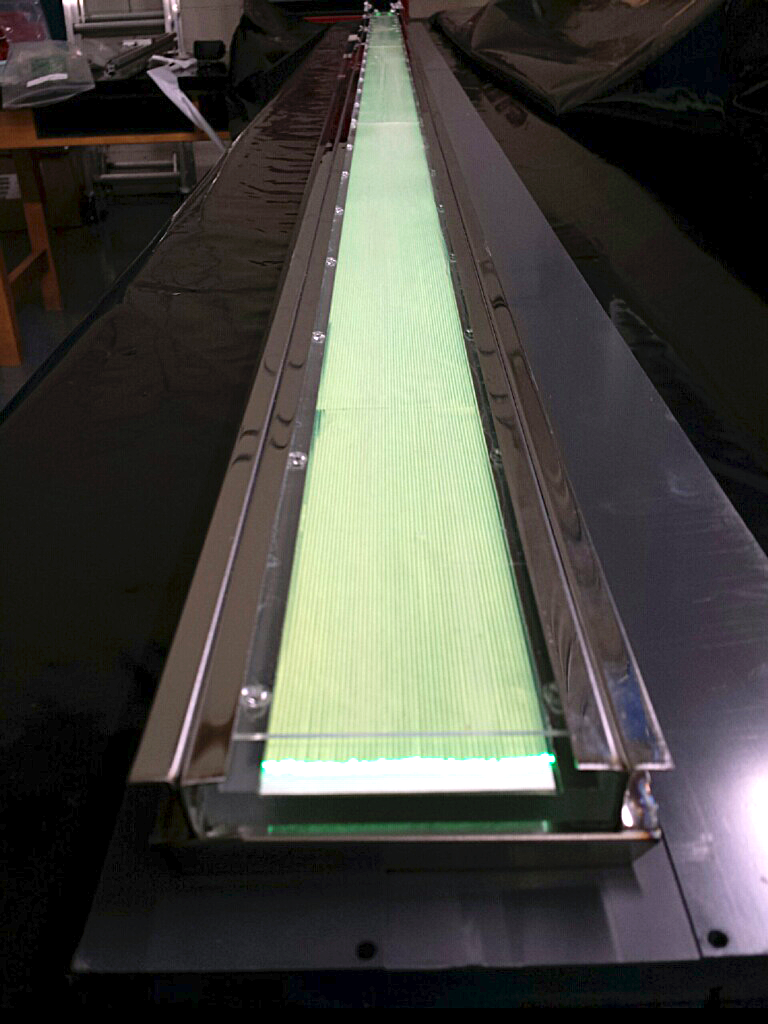
\includegraphics[width=.6\columnwidth]{fiber_bundle_1.png}
\caption{Photograph of fiber-bundle PD prototype (early 1-sided
  version). The thin TPB-coated radiator is mounted on top of the
  prototype in the image.}
\label{fiber_bundle}
\end{figure}

The VUV photons are incident on the TPB-coated plastic radiator and
roughly ½ of the photons converted in the radiator are incident on the
bundle of fibers, which are directed onto SiPMs at one end. The Y11
fiber (from Kuraray ) have mean absorption and emission wavelengths of
about 440 nm and 480 nm respectively.  The attenuation length of the
Y11 fibers is given to be greater than 3.5 m at the mean emission
wavelength, which allows production of full-scale (2.2 m length)
photon detector paddles.  

Another benefit of this design is that the fibers could be arranged
into two rows with each row of fibers collected onto individual
SiPMs. If back-to-back reflectors were to be inserted between the rows
of fibers each row would then face into different TPC cells allowing
additional information to be used in the disambiguation of the TPC
signals coming from wire wrapping on the APA frames. A further benefit
of the design could be compatibility with concepts where the walls of
the detector are covered with TPB coated material shifting the VUV
photon to blue and then the WS-fiber can capture the emitted light.


\section{SiPM}

\section{Photon system readout electronics}
\label{sec_elec}

Scintillation light from LAr comes from the two different excited
states with lifetimes of about 6 ns and 1.6 $\mu$s.  Only a limited
amount of light is collected by this system, so the electronics must
be designed to collect the light from both excited states. A summary
of the general requirements for the system, including requirements
from a physics performance perspective, are given in
Table~\ref{tab:fee_req}.
%
\begin{table*}[ht]
\centering
%\vspace{4mm}
\begin{tabular}{| l | l |} \hline
 Performance Parameter       & Target   \cr   \hline
 Time Resolution                   & Better than 30 nS wrt event time zero ("t0")      \cr  \hline
 Charge Resolution               & 0.25\% photo-electron equivalent                     \cr \hline
 Dynamic Range                   & $\sim$ x10 better than detector (1000:1)          \cr \hline
 Linearity                               & Sufficient to resolve 1 photo-electron signals   \cr    \hline
 Multi-Hit Capability              & Sufficient to measure Triplet (late) Photons          \cr   \hline
 Dead Time                           & Live up to 2 drift times either side of beam spill          \cr    \hline
 Bias Control                        & 0.1 V resolution up to 30 V per channel  \cr    \hline
 Calibration                          & On-board Charge Injection  \cr    \hline
 Timing                                 & Events time-stamped using NO$\nu$A Timing syst.  \cr    \hline
\end{tabular}
\caption{\label{tab:fee_req} Physics Requirements for the Photon Detector Electronics.}
\end{table*}
%
The plans for the electronics for the photon detection subsystem
include a baseline design with several options that remain R\&D
activities.  There alternative implementations of electronics are
described in Section~\ref{sec_alt}.
%These options are identified in the description that follows.  
%There are also some alternative implementations of electronics that remain under consideration.  These are described in Section~\ref{sec_alt}
%These are described in Section 6.4.

In the baseline plan, there are no front-end electronics in the cold
volume.  Instead, the un-amplified signals from the SiPMs are
transmitted to outside the cryostat on cables for processing and
digitization, as shown in Fig.~\ref{fig:fig-e-1}.  There are
advantages and disadvantages to this approach.  The advantages are
that the infrastructure required for inside the cryostat is reduced
(power, data cables, precision clocks, data protocols, etc.);
reliability is improved (no single-point failures of multi-channel
devices inside the cryostat); serviceability and accessibility to the
front-end electronics are improved; and the need to develop cold
electronics, possibly a custom ASIC, is eliminated.  The disadvantages
are that the cable plant inside the detector is increased, which can
create mechanical challenges and installation difficulties; the flange
board (warm/cold interface) is more complex; there are generally more
connectors in the system; and signal-to-noise considerations are more
difficult.  Generally, the baseline design favors simplicity,
reliability and reduced R\&D time and costs, and also meets the
performance requirements of the electronics.
%
 \begin{figure}[h]
  \centering
%\includegraphics[angle=0,width=10cm,height=7cm]{fig1}
\caption{Block diagram of the photon detector signal processing system.}
\label{fig:fig-e-1}
\end{figure}
%
In the 35-ton prototype, each SiPM signal was transmitted on an
individual shielded twisted-pair cable fitted with individual
LEMO-style connectors.  The bias voltage was coupled onto the signal
cable, using AC-coupling on the receiving end to measure the SiPM
signal.  The use of high-quality cable with point-to-point connections
between an individual SiPM inside the cryostat and the front-end
electronics residing outside the cryostat, combined with good
differential signal processing on the receiving end, enabled the
demonstration of the principle that single photo-electron signals
could be measured accurately without the need for cold electronics.
In order to address the problems with the cable plant as identified
above, the following ideas are being pursued:
\begin{itemize}
\item Ganging together of several SiPM outputs from a given PD
  detector into one output cable.  This increases the detector
  capacitance, affects the pulse shape, and could spoil the timing
  resolution of the measurement.  Also, the SiPMs may have to be
  preselected, since there will be only one bias voltage for three
  devices, and it may be important to match the over-voltage
  characteristics.  Studies are in progress to find a compromise
  between data precision and cabling issues. One approach is to add a
  cold pre-amplifier if the ganging together of several SiPMs result
  in performance that is too degraded to meet specifications.  The
  infrastructure requirements (cables, connectors, power, cold
  performance, reliability, mechanical mounting, etc.) would have to
  be considered.

\item Use of multi-conductor, individually shielded pair cable.  A candidate cable containing four individually-shielded twisted pairs has been 
identified and tests are in progress.  The cable is in Teflon jacket, which should be acceptable for use in LAr.

\item Use of mass-terminated connectors.  Several candidate connectors
  for use with the cable described above are being pursued.
\end{itemize}

The baseline plan assumes that three SiPM signals can be ganged
together into one readout channel.  By using the multi-conductor cable
with four twisted pairs, this results in one cable per PD consisting
of 12 SiPMs.  The diameter of this cable is ~xxx mm, which reduces the
cable plant by $\sim$ x10 compared to that used in the 35 ton
detector.  The cost of the connectors also decreases by $\sim$ x10.
Lastly, the ease in making connections at the flange board will be
improved by the use of a mass-terminated connector.

In the baseline plan, the front-end electronics resides outside of the
cryostat in instrumentation racks.  We have designed and built a
custom module for receiving SiPM signals, and performing signal
processing in the front-end as preprocessing for trigger and DAQ.  The
module is called the SiPM Signal Processor (SSP).  An SSP consists of
12 readout channels packaged in a self-contained 1U module.  Each
channel contains a fully-differential voltage amplifier and a 14-bit,
150 MSPS analog-to-digital converter (ADC) that digitizes the
waveforms received from the SiPMs.  The front-end amplifier is
configured as fully-differential with high common-mode rejection, and
receives the SiPM signals into a termination resistor that matches the
characteristic impedance of the signal cable.  Currently there is no
shaping of the signal, since the SiPM response is slow enough relative
to the speed of the digitization to obtain several digitized samples
of the leading edge of the pulse for the determination of signal
timing.

The digitized data is stored in pipelines in the SSP, for up to $\sim$
13 $\mu$s.  The processing is pipelined, and performed by a Xilinx
Artix-7 Field-Programmable Gate Array (FPGA).  The FPGA implements an
independent Data Processor (DP) for each channel.  The processing
incorporates a leading edge discriminator for detecting events and a
constant fraction discriminator (CFD) for sub clock timing resolution.
Because the FPGA is programmable and accessible, it is possible to
explore different data processing algorithms and techniques, and even
customize the readout for a given type of event (supernova for
example.)  A picture of the module is shown in Fig.~\ref{fig:fig-e-2}.
A block diagram of the system is shown in Fig.~\ref{fig:fig-e-3}.
%Fig. xx3.  Picture of the SSP module.
%
\begin{figure}[h]
  \centering
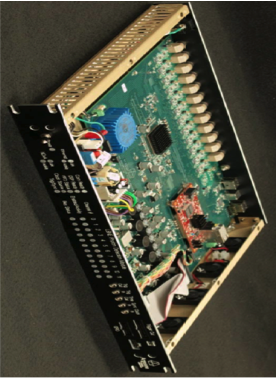
\includegraphics[angle=90,width=10cm,height=5cm]{fig-e-2.png}
\caption{Picture of the SSP module.}
\label{fig:fig-e-2}
\end{figure}
%
%Fig. xx2.  Block diagram of the SSP.
%
\begin{figure}[h]
  \centering
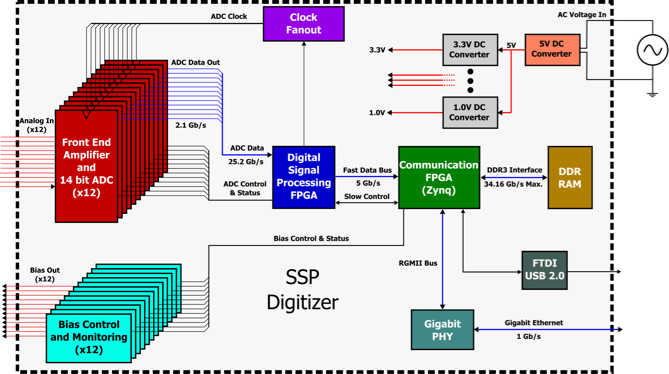
\includegraphics[angle=0,width=12cm,height=7cm]{fig-e-3.png}
\caption{Block diagram the SSP module.}
\label{fig:fig-e-3}
\end{figure}
%
In the simplest mode of operation, the module can perform waveform
capture, using either an internal trigger or an external trigger.  Up
to 2046 waveform samples may be read out for each event.  When
waveform readouts overlap the device can be configured to offset,
truncate or completely suppress the overlapping waveform.  Pile-up
events can also be suppressed.

As an alternative to reading full waveforms, the DP can be configured
to perform a wide variety of data processing algorithms, including
several techniques for measuring amplitude, and also timing of the
event with respect to a reference clock.  All timing and amplitude
values are reported in a compact event record.  Each data processing
channel stores up to 340 event records when not storing waveforms.

Generally, the SSP performs pipelined processing.  The module has been
designed to support several different triggering schemes, including
self-triggered, use of an external trigger, or use an external gate to
readout all events within a time-window.  In order for the events
measured in the photon detector to be matched up with the
corresponding events in the TPC, the front-end electronics attaches a
timestamp to the data as it is acquired.  The timestamp is unique, and
has a correspondence with the timestamps in the TPC electronics
processing.  The timestamp in the SSP is applied to the event data as
it is digitized, and becomes part of the data as the processing
proceeds.  In the case where zero-suppression and data sparsification
are used, the timestamp on accepted data remains intact.  To achieve
this, the TPC and PD electronics must be synchronized, including
timestamp counter resets, and a known and stable calibration between
the corresponding timing resolution of the ADC conversion in the two
systems.  The electronics has been designed to support a full
interface to the NO$\nu$A timing system, which is the baseline timing
system for the experimental prototypes.

A Xilinx Zynq FPGA, onboard the MicroZed system-on-module, handles the
slow control and event data transfer.  The SSP has two parallel
communication interfaces; USB 2.0 and 10/100/1000 Ethernet.  The 1
Gb/s Ethernet supports full TCP/IP protocol.  The module includes a
separate 12-bit high-voltage DAC for each channel to provide up to 30
V of bias to each SiPM.  The module also feature charge injection for
performing diagnostics and linearity monitoring, and also voltage
monitoring.

In tests to date, the SSP is capable of measuring single
photo-electron signals coming from the SiPMs over a cable length of 30
meters when the SiPMs are operated at LAr temperatures.  The timing
resolution of the signals has been measured to be better than 3 ns.
The full-differential signal processing in the front-end circuitry is
important in achieving this result.
 
The SSP is self-contained in that it receives 60 Hz, 120V power, and
has internal linear and DC/DC power supplies for generating the DC
voltages needed for the instrumentation, as well as the bias voltage
for the SiPMs.  The SSP is packaged in a 1U, rack-mountable
package. For the 35-ton prototype, the racks are located near the
ports on the top of the cryostat.

\subsection{Alternatives}
\label{sec_alt}

In the baseline design of the PD electronics, the approach was taken
to have no electronics inside of the cold volume.  This results in a
large number of cables and connectors.  Other experiments using liquid
argon have successfully implemented cold TPC electronics, thereby
significantly reducing the cable plant that must come through the
cryostat.  This approach has challenges in power distribution, heat
dissipation, and the performance of front-end electronics in LAr. To
address serviceability, the cold electronics might be realized in a
modular way and situated just below the flange in the cryostat so that
it can be accessed in the event that repair is needed.  To this end
the zero-suppression will be important to avoid high data rates
depending on the number of readout channels needed. A way to realize
the cold zero-suppression would be to implement a cold FPGA (or an
ASIC, yet to be developed).  So far the cold FPGAs have had mixed
results in tests. Alternative approach would be to perform an "analog
zero suppression" with a constant-fraction discriminator and then gate
the signal and digitize warm, in which case the complication with
encoding the particular channel has to be addressed.  The significant
challenges in this technique include power dissipation, the increased
possibility of contamination of the LAr, and extended infrastructure
requirements that must reside in the cold volume.  The virtue is that
this can significantly reduce the number of signal penetrations into
the cold volume.

The electronics for the photon detector of LBNE uses fast (direct)
digitization of the SiPM pulses. Another option for the front-end
electronics is to use pulse shaping. Instead of digitizing the full
bandwidth of the SiPM signal, the pulse is shaped using analog
filtering techniques, generally producing a pulse with a prescribed
shape with a peak that is proportional to the total amount of charge.
By measuring the peak, both amplitude and pulse timing can be
obtained.  Since the pulse response follows a known transfer function,
the pulse peak can be obtained using slower synchronous sampling, or
using asynchronous sampling through the use of peak detection and
constant fraction discrimination.  In either case, the data can be
processed by an FPGA, using algorithms optimized for the application.
In particular, assuming that a sufficient number of samples are
obtained of the shaped pulse, a chi-square comparison of the shape to
the ideal pulse can be used to determine pulse corruption, or event
identification.  As with direct digitization, the digitization clock
and timestamp can be synchronized using an external clock source. The
data can be read out in a similar manner, using USB 2.0 or 10/100/1000
Ethernet.  The virtue of this approach is that a slower ADC can be
used, reducing power consumption, and also reducing data load and the
speed of readout links.  The technique does trade bandwidth for
shaping, making timing and pile-up issues more important.  This can
result in the interpretation of the pulse shape becoming more complex
than direct digitization.  Generally, the pulse shaping circuitry is
also less expensive than the direct digitization technique, assuming
similar performance requirements.

Another option for the photon system readout would include the use use
of an Application Specific Integrated circuit (ASIC) as a way to
reduce cost.  The large channel count in a real detector system is
such that the production cost of the system could be greatly reduced.
Often, the cost of development of an ASIC from scratch is quite high,
of order $\sim$400K, and can take ~1-2 years for development, so cost
and schedule must be weighed carefully.  However, other benefits from
the ASIC approach include reduced space requirements for circuitry on
the front-end, lower power dissipation, and specialized functionality
in the front-end chip.  There exist several ASICs that have been
designed over the last few years especially for SiPM readout.  One
could potentially explore the functionality and performance of these
designs, and evaluate their suitability for LBNE.  This option might
be used either for warm or cold electronics.  Direct digitization has
the virtue of being straight-forward from a circuit design
perspective.  By taking advantage of modern high-bandwidth OP amps,
high-speed, high-rate ADCs, and powerful FPGAs with high-speed serial
links, it is possible to obtain 14-bit dynamic range digitization with
$\sim$1 ns timing resolution.  By reading all of the samples into an
FPGA having a deep buffer, digital signal processing techniques can be
employed using the programmable logic, offering powerful analysis
algorithms that can be developed in time.  The technique generally has
higher power consumption and tends to be more expensive than simpler
instrumentation techniques.

\section{Photon Detector Calibration}
\label{sec_pd_calib}

The photon detector calibration is a part of a larger calibration plan
that covers all aspects of an LAr detector calibration, and includes
methods to convert collected charge to initial particle?s energy, as
well as calibration techniques to convert collected scintillation
light into estimate of particle's interaction time, energy, and a
track/vertex location for each event.  As already described, the
baseline for the scintillation photon detectors assumes employment of
acrylic light collection paddles to reduce the required costly
photo-cathode area. Several photon detector designs are presently
being developed and are being tested in small dewars. Since each of
these new elements has not yet been tested in a large-scale TPC, the
35-ton LArTPC prototype is being constructed to provide essential
design validation. The current FD designs are anticipated to have
sufficient sensitivity to provide event timing information for
atmospheric neutrino and proton decay channels. However, it will not
provide high efficiency down to the 5 MeV neutrino energy level
desired by the supernova program. This would have the impact that the
event reconstruction energy resolution would be 20\% rather than 5\%
achievable with the event time determination from a photon detector
able to operate efficiently at a sufficiently low energy
threshold. The improvement in physics will be studied in the near
future but a substantial effort in development of improved detection
techniques is desired. In the absence of precise physics requirements
for the photon detector system and in order to support R\&D activities
on the photon detector development it was decided that the photon
detector should provide a time stamp to determine the time of
occurrence of an event (so called ?time zero?) with an accuracy much
better than 1 ?s.  Items relevant to the photon detector calibration
are the fast and slow components of the light, photon propagation
including scattering and reflections, impact of N2, E-field strength,
as well as the energy range of interest. A calibration system that
addresses the issues listed above has to be both comprehensive and
cost-effective, and has to be tied to the overall calibration system
that includes both charge and scintillation light calibration
techniques. Such a system will be designed in the future.  To support
the PD R\&D phase we designed a light-flasher based calibration system
that will serve to monitor the relative performance and time
resolution of the system. In particular, for anticipated 35-ton
performance tests we need to evaluate relative efficiencies of
multiple light collection techniques in order to be able to
down-select an optimal light readout technology. The system that meets
these requirements will consist of a set of LEDs as light sources or a
laser with a VUV wave-length, coupled to quartz fibers, thus
transmitting light from outside the detector volume to desired
locations at the CPA within a TPC. Therefore we will equip the 35-ton
detector with LEDs located and fired externally, with fibers running
into the cryostat, to diffusers that will emit light from the CPA to
the APA. For the 35-ton cryostat at the surface at Fermilab it will be
complementary to cosmic ray muon tracks as means of calibration. In
terms of light sources the measurements should be performed with an UV
(245-375nm) light source. The UV light mimics physics starting from
the wavelength shifter conversion, light guide propagation,
photo-sensor detection and FEE readout.  The external light-flasher
calibration system is designed under following assumptions:
\begin{itemize}
\item simple to implement (no active components within PD/APA, such as
  LEDs or fibers mounted within APA).
\item less-intrusive (less material within detector in terms of
  fibers, then equipping each PD frame with individual fiber).?\item
  provide a benchmark light-based reconstruction with the use of
  localized light sources distributed throughout the detector volume.
\item has a potential to be adapted for deployment in a large Far
  Detector in the future
\end{itemize}

We describe the system in Fig.~\ref{fig:fig-c-1}. . The system
consists of a 1U rack mount Photon Detector Calibration Module (PDCM)
sitting outside the liquid argon cryostat. The module generates light
pulses that propagate through a quartz fiber-optic cable to diffusers
at cathode-plane (CPA) to distribute the light uniformly across the
photon detectors mounted within anode plane (APA).  There are 5
diffusers on the CPA plane: one in the center and four diffusers close
to the CPA corners, as shown in Fig.~\ref{fig:fig-c-2}. .
%
 \begin{figure}[h]
  \centering
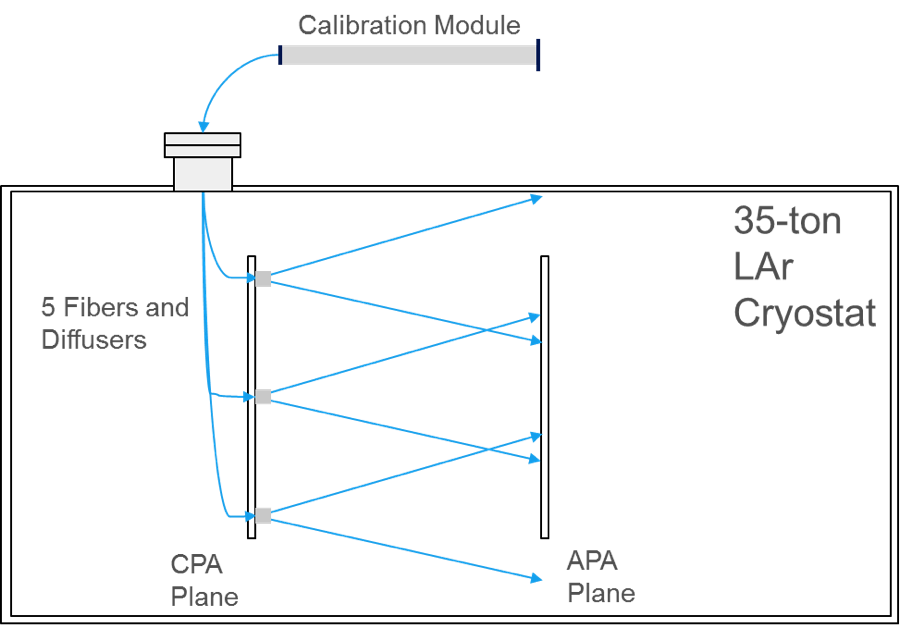
\includegraphics[angle=0,width=10cm,height=7cm]{fig-c-1.png}
\caption{Concept of the UV-light calibration system for the photon
  detector in liquid argon.}
\label{fig:fig-c-1}
\end{figure}
%
?%
 \begin{figure}[h]
  \centering
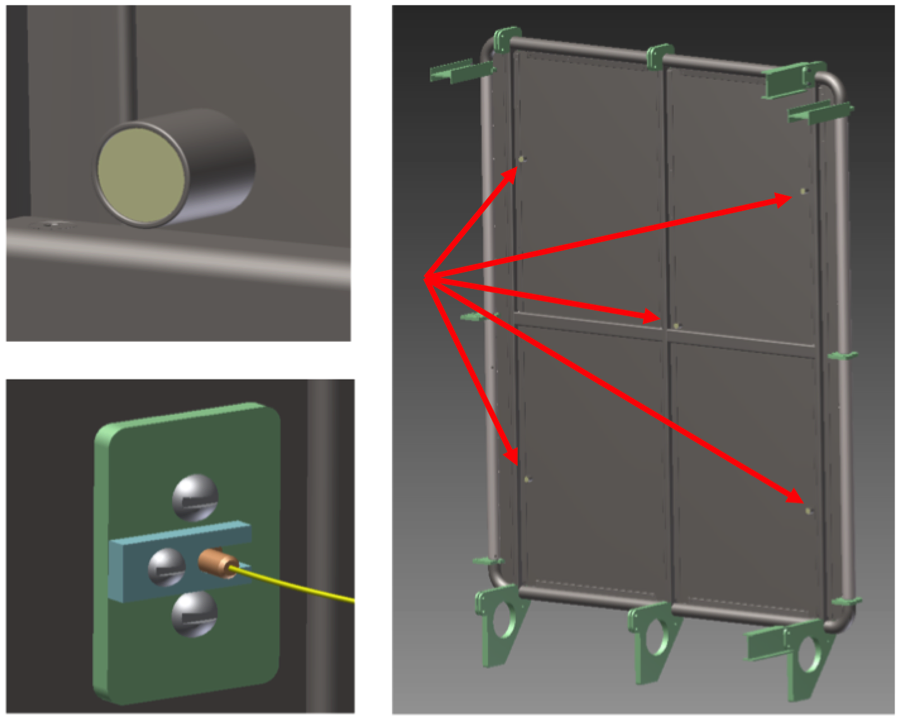
\includegraphics[angle=0,width=10cm,height=7cm]{fig-c-2.png}
\caption{The diffuse light is emitted from diffusers (top left figure)
  mounted at five CPA locations, indicated by arrows (right figure).
  The UV light from the PDCM to diffusers is transported through
  quartz fiber (lower left figure).}
\label{fig:fig-c-2}
\end{figure}
%

The PDCM module layout is shown in Fig.~\ref{fig:fig-c-3}. The ANL
photon calibration module is based on a re-purposed SSP unit.  An SSP
board will be repackaged into a deeper rack mount chassis that will
accommodate a new internal LED Pulser Module (LPM) and an additional
bulk power supply. The LPM utilizes five digital outputs to control
the LPM pulse and its duration (arrows in black).  These LVDS outputs
are derived from the charge injection control logic within the SSP?s
FPGA.  The even channel SiPM bias DACs are repurposed to control the
LPM pulse amplitude (arrows in red).  The adjacent odd channels are
used to readout a photodiode which is used for pulse-by-pulse
monitoring of the LED light output.  The output of the monitoring
diode is used to normalize the response of the SiPMs in the detector
to the calibration pulse

%
 \begin{figure}[h]
  \centering
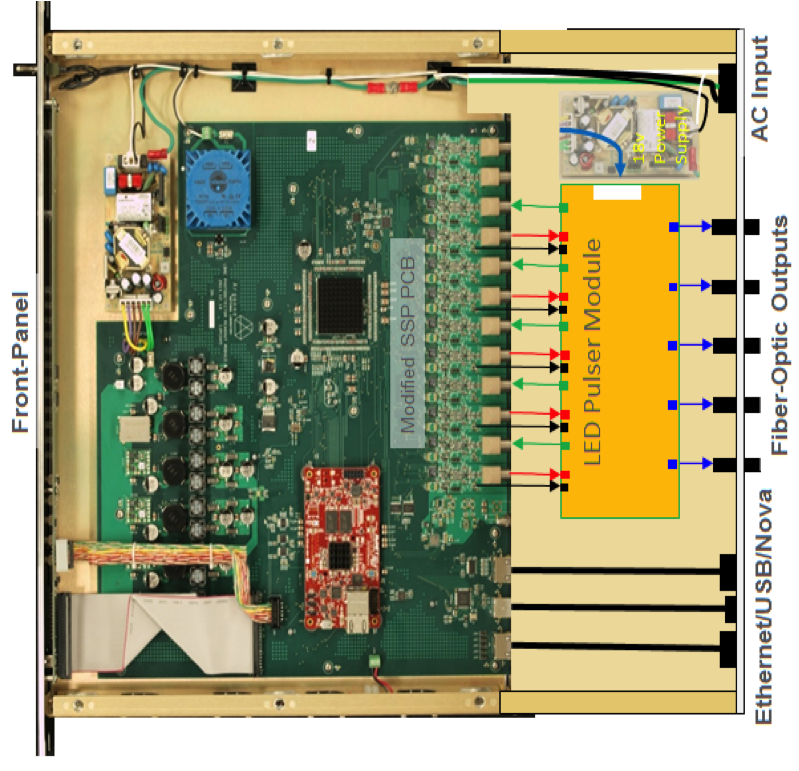
\includegraphics[angle=0,width=10cm,height=7cm]{fig-c-3.png}
\caption{Photon detector calibration module (PDCM) layout.}
\label{fig:fig-c-3}
\end{figure}
%

For the 280 nm light we have performed a simulation of the designed
diffuse light calibration system using TracePro, a generalized 3-D
light ray-tracing program with the ability to include bulk optical
properties such as absorption, fluorescence, birefringence in addition
to surface properties such as scattering and
reflection. Fig.~\ref{fig:fig-c-4} shows simulated light distributions
of at the 35-ton APA for the cases of the VUV light emitted by either
the central diffuser only (left figure), or by outer four diffusers
simultaneously (right figure). A full Geant4 based simulation of the
detector will be used in the future. Using the preliminary data with
the 35-ton style light guides (indicating 0.5\% efficiency for number
of photo-electrons per incident 128 nm LAr scintillation photon 50 cm
from the light guide), we estimate for 280 nm light to observe ~15
photo-electrons per single SiPM channel when the light is emitted from
the single central diffuser in 13 ns long pulses. Similarly, we expect
about ~100 photo-electrons observed by a single SiPM channel when 280
nm light is emitted in 100 ns long pulses from the four outer
diffusers at once.

%
 \begin{figure}[h]
  \centering
  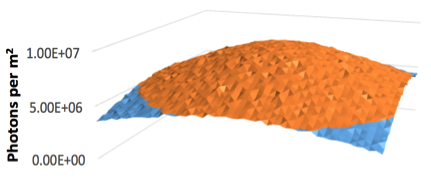
\includegraphics[angle=0,width=6.5cm,height=3.5cm]{fig-c-4-L.png}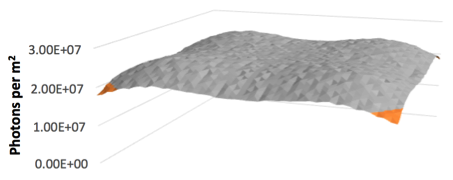
\includegraphics[angle=0,width=6.5cm,height=3.5cm]{fig-c-4-R.png}
\caption{Simulated light distributions of at the 35-ton APA for the
  cases of the VUV light emitted by either the central diffuser only
  (left figure), or by outer four diffusers simultaneously (right
  figure).}
\label{fig:fig-c-4}
\end{figure}
%

In the LBNE prototypes (i.e. in 35-ton) and in Future Far Detector it
will be important to check if photon-detector components are
functioning properly at various stages of the detector
operation. Periodic light source deployments will monitor the systems
stability as a function of time. A change in relative difference of UV
light responses will indicate towards potential wave-length shifter
instability, changes in SiPM gain and collection efficiencies. Much of
the same monitoring is expected to be doable with cosmic rays in the
35-ton (at surface), with periodic LED/laser calibration runs
complemented with cosmic-ray data tracked with an external
hodoscope. With the 35-ton detector one could use a well-defined muon
trajectory defined by the hodoscope geometry and monitor the number of
PEs per MeV of deposited charge. The number of PEs per PD channel from
the well-defined muon track could be used as a calibration
constant. However, for the deep underground LBNE the cosmic ray flux
may inadequate for timely monitoring of the photon detectors.  With
the 35-ton detector we have planned two sets of calibration runs:
\begin{enumerate}
\item Calibration runs with four outer diffusers run simultaneously,
  in order to\\ -measure response of PD channels in multi-PE range and
  get integrated number of event samples for each channel (for maximum
  light output)\\ -test of the dynamic range from 1PE to maximum
  number of PEs. \\ -repeat runs periodically to trace any changes in
  channel response.
       
\item Runs with central diffuser only, in order to\\ -perform initial
  calibration runs that will reveal malfunctioning channels, if
  any.\\ -timing measurements with the 10-50 ns pulses, verify time
  resolution of the PD system.
\end{enumerate}

The controlled source of light described here will be used to perform
a relative ?t0? calibration, where the ?t0? could be absolutely
calibrated with the use of the cosmic ray triggers available with
35-ton detector. Effects that contribute to a finite time resolution
and relative time offset of PD channels include scintillation time
constants, photon conversion with wave-length shifter, photon
propagation through PD paddle, SiPM jitter, and FEE resolution. Most
these effects are constant and can be individually measured on the
bench, so the LED flasher system will monitor overall stability of the
photon detector.  To go beyond the current R\&D phase one needs
detailed MC simulations of light production, propagation, and
detection to perform comparisons of reconstruction performance against
prototype data in terms of calorimetric energy and position
reconstructions for measured event tracks. Future light collection
systems will aim to maximize the active area of the light guide bars,
to achieve a high photon detection efficiency with an optimized timing
and granularity required for improved position resolution. As in the
case with the TPC charge calibration we will need to evaluate what may
be achieved with expected cosmic ray muons and Michels, $\pi^0$, and
natural radioactivity events (such as $^{39}$Ar with end-point energy
of abut 500 keV).


\section{Installation}







